\chapter{Gráficos del análisis preliminar de métricas}
\label{cap:gapm}


En este anexo se exponen los gráficos obtenido de la proyección del resultado obtenido de la detección tanto para el eje \textit{y} como para el eje \textit{x}.

\section{Gráficos de proyección de la matriz resultado}

\begin{figure}[H]
  \centering
  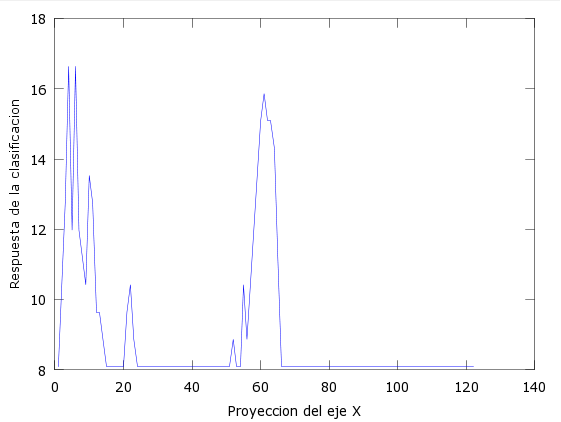
\includegraphics[scale=.4]{images/plots/boost1X}
  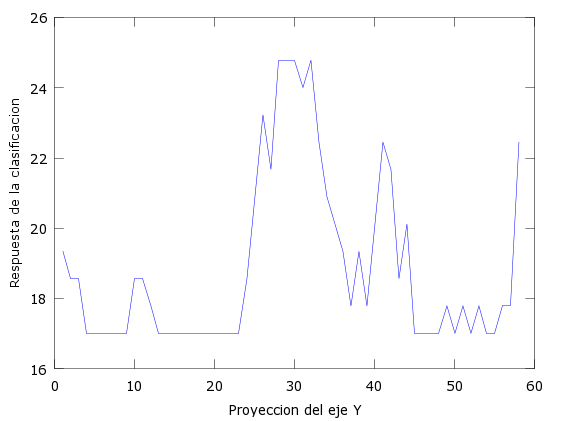
\includegraphics[scale=.4]{images/plots/boost1Y}
  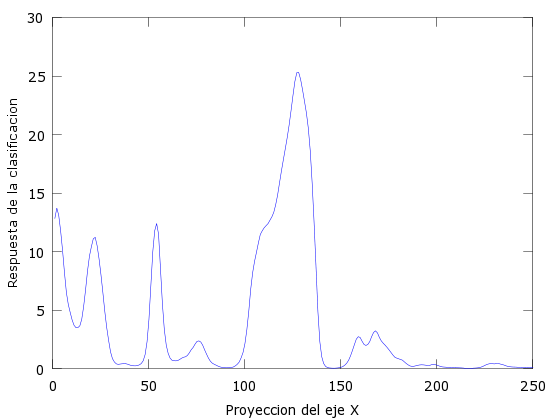
\includegraphics[scale=.4]{images/plots/svm1X}
  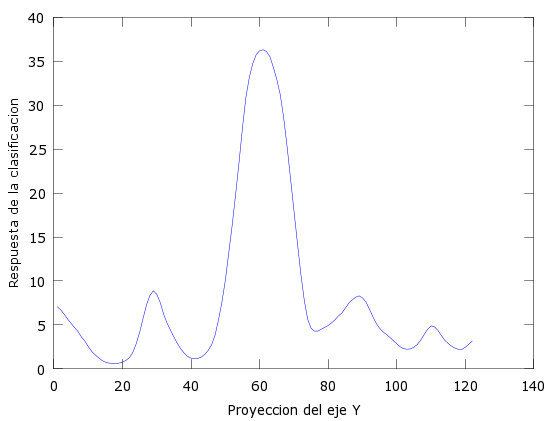
\includegraphics[scale=.4]{images/plots/svm1Y}
  \caption{\em  Proyección de ejemplo de resultados.A la izquierda, proyección en el eje x. A la derecha, proyección en el eje y. Arriba Adaboost. Abajo SVM}     
  \label{fig:pro1}
\end{figure}

\begin{figure}[H]
  \centering
  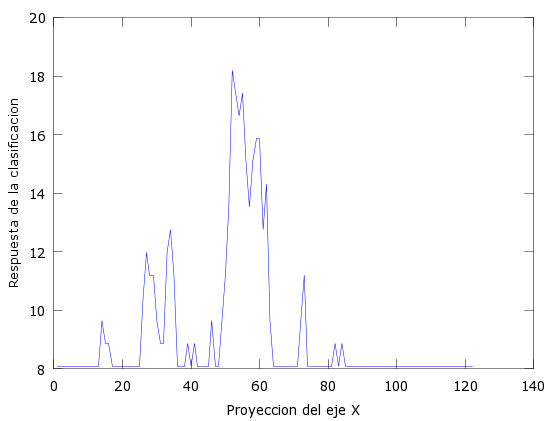
\includegraphics[scale=.4]{images/plots/boost2X}
  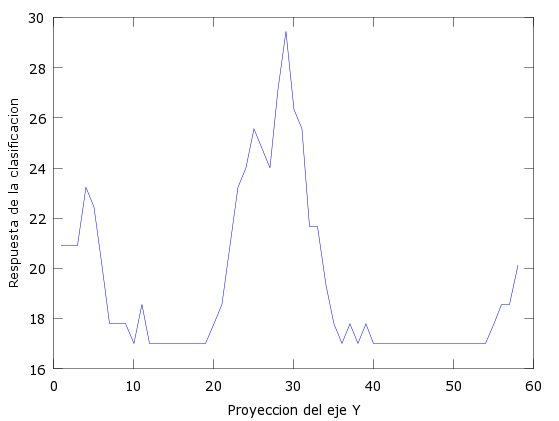
\includegraphics[scale=.4]{images/plots/boost2Y}
  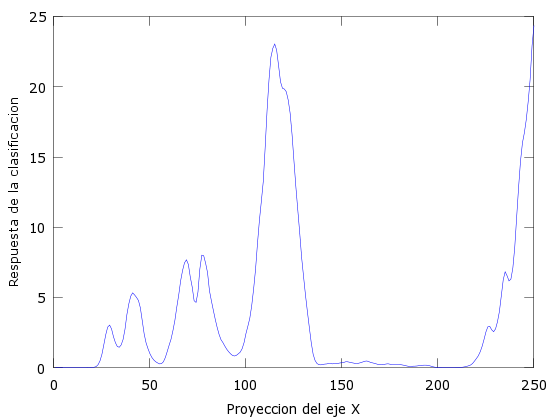
\includegraphics[scale=.4]{images/plots/svm2X}
  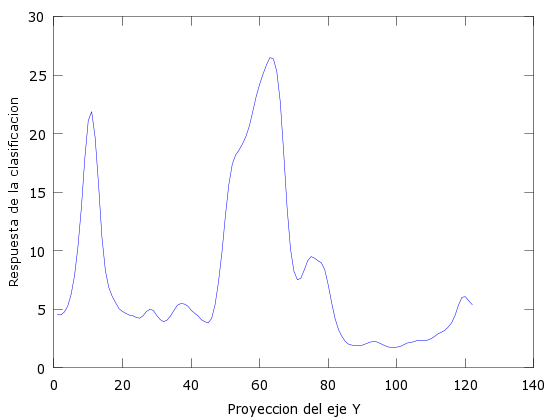
\includegraphics[scale=.4]{images/plots/svm2Y}
 \caption{\em  Proyección de ejemplo de resultados.A la izquierda, proyección en el eje x. A la derecha, proyección en el eje y. Arriba Adaboost. Abajo SVM}   
 \label{fig:pro2}
\end{figure}
\begin{figure}[H]
  \centering
  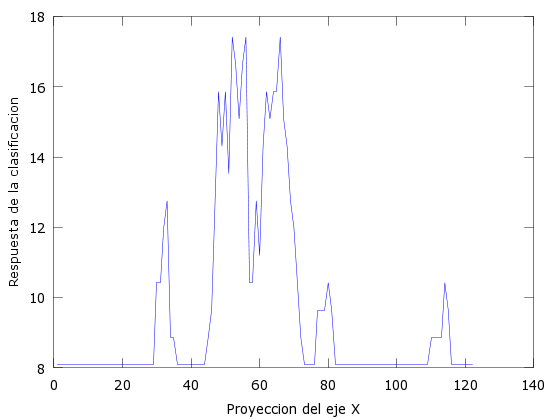
\includegraphics[scale=.4]{images/plots/boost3X}
  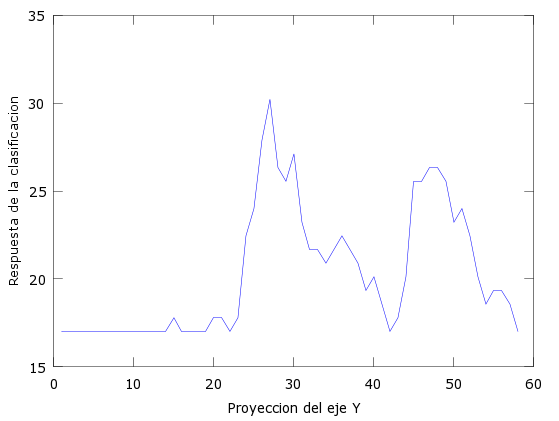
\includegraphics[scale=.4]{images/plots/boost3Y}
  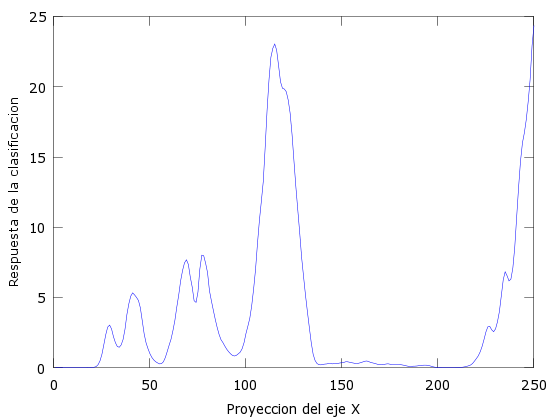
\includegraphics[scale=.4]{images/plots/svm2X}
  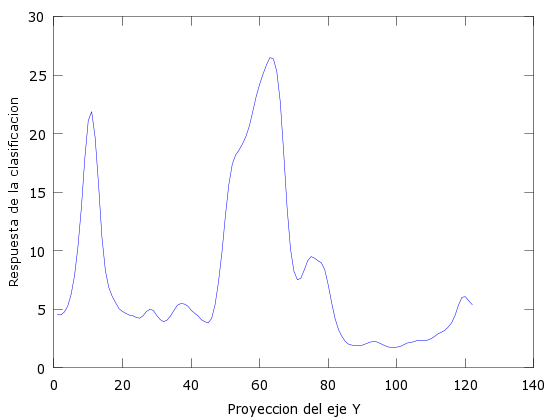
\includegraphics[scale=.4]{images/plots/svm2Y}
\caption{\em  Proyección de ejemplo de resultados.A la izquierda, proyección en el eje x. A la derecha, proyección en el eje y. Arriba Adaboost. Abajo SVM}   
\label{fig:pro3}
\end{figure}
\begin{figure}[H]
  \centering
  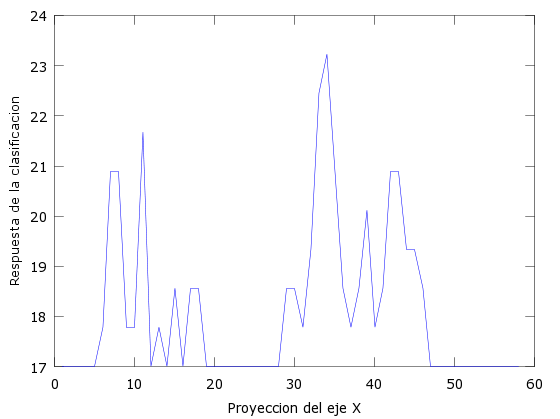
\includegraphics[scale=.4]{images/plots/boost4X}
  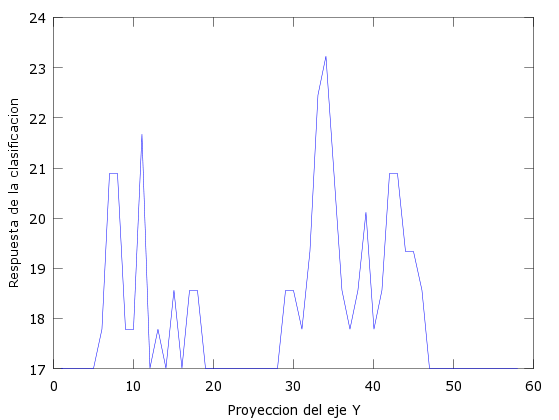
\includegraphics[scale=.4]{images/plots/boost4Y}
  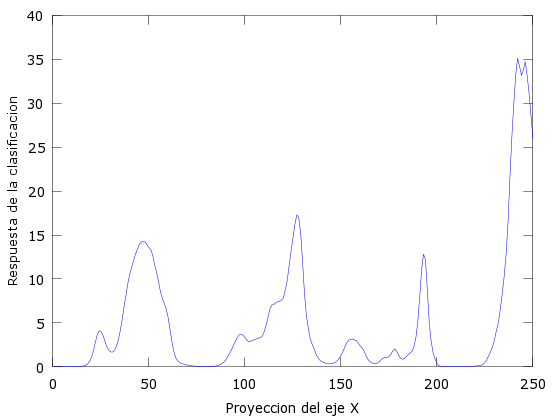
\includegraphics[scale=.4]{images/plots/svm4X}
  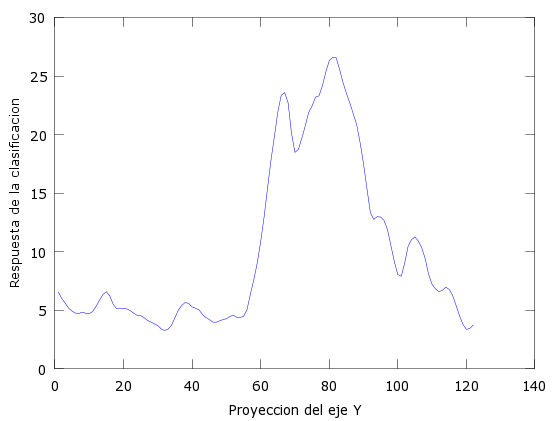
\includegraphics[scale=.4]{images/plots/svm4Y}
 \caption{\em  Proyección de ejemplo de resultados.A la izquierda, proyección en el eje x. A la derecha, proyección en el eje y. Arriba Adaboost. Abajo SVM}   
 \label{fig:pro4}
\end{figure}
\begin{figure}[H]
  \centering
  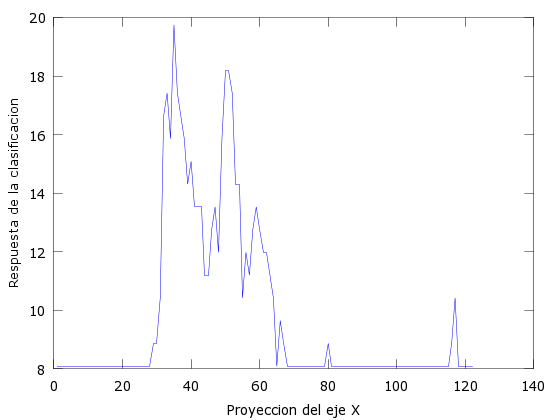
\includegraphics[scale=.4]{images/plots/boost5X}
  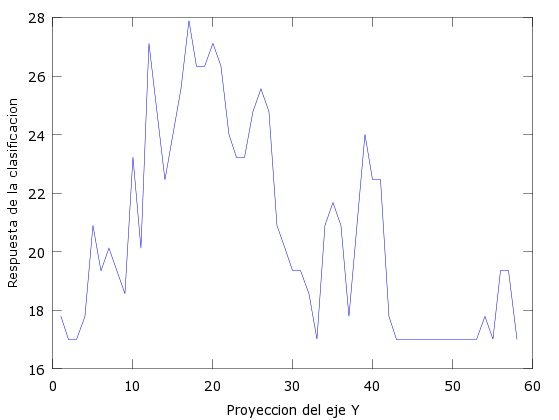
\includegraphics[scale=.4]{images/plots/boost5Y}
  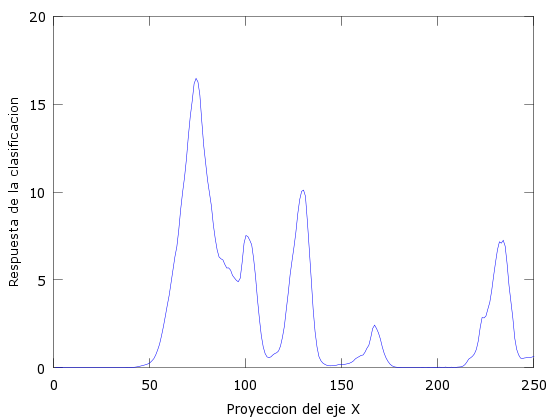
\includegraphics[scale=.4]{images/plots/svm5X}
  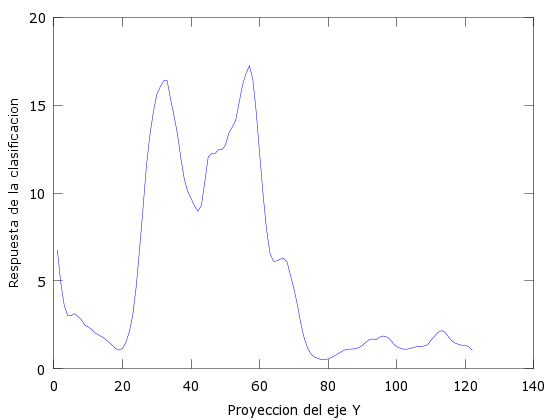
\includegraphics[scale=.4]{images/plots/svm5Y}
 \caption{\em  Proyección de ejemplo de resultados.A la izquierda, proyección en el eje x. A la derecha, proyección en el eje y. Arriba Adaboost. Abajo SVM}   
 \label{fig:pro5}
\end{figure}
\begin{figure}[H]
  \centering
  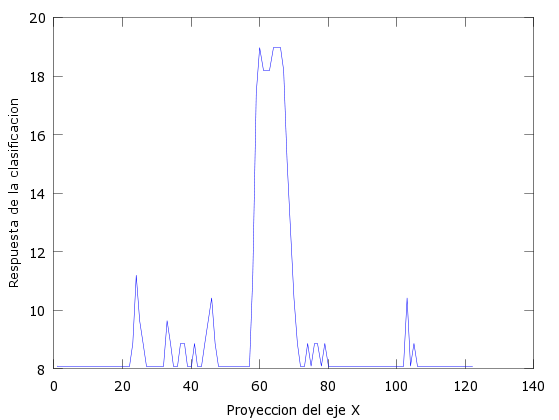
\includegraphics[scale=.4]{images/plots/boost6X}
  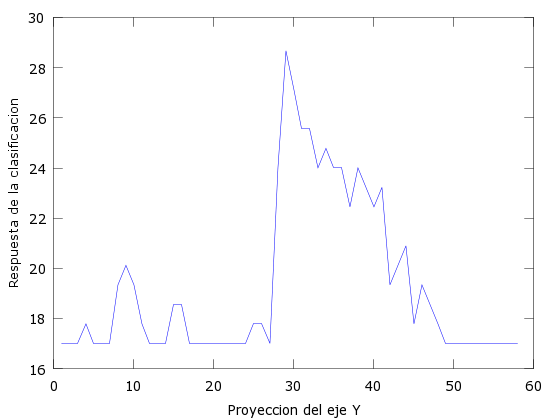
\includegraphics[scale=.4]{images/plots/boost6Y}
  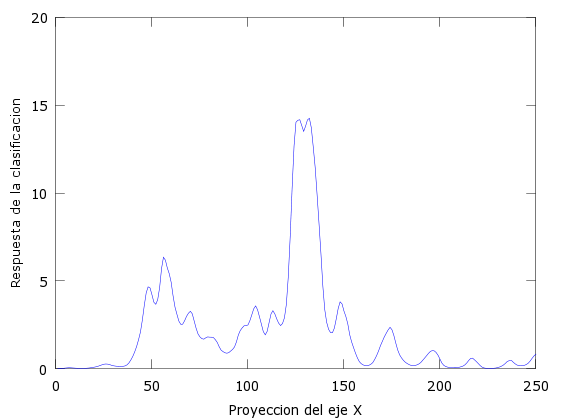
\includegraphics[scale=.4]{images/plots/svm6X}
  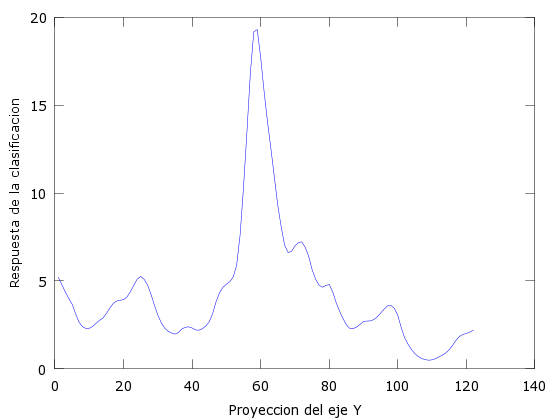
\includegraphics[scale=.4]{images/plots/svm6Y}
  \caption{\em  Proyección de ejemplo de resultados.A la izquierda, proyección en el eje x. A la derecha, proyección en el eje y. Arriba Adaboost. Abajo SVM}   
  \label{fig:pro6}
\end{figure}
\begin{figure}[H]
  \centering
  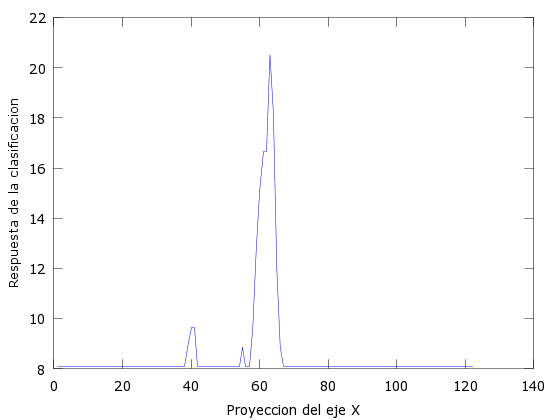
\includegraphics[scale=.4]{images/plots/boost7X}
  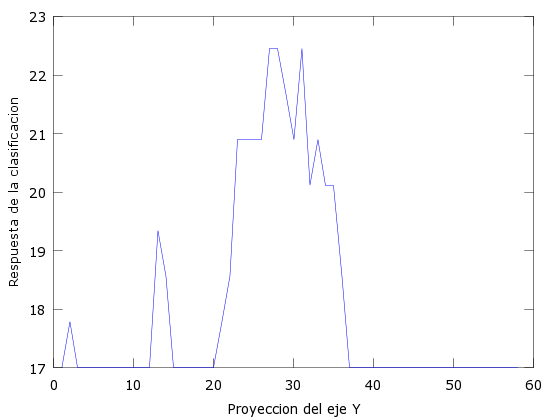
\includegraphics[scale=.4]{images/plots/boost7Y}
  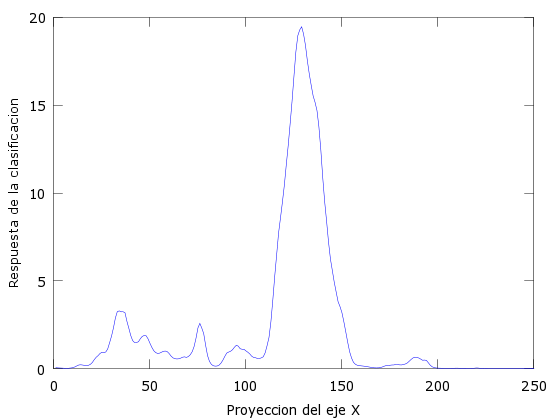
\includegraphics[scale=.4]{images/plots/svm7X}
  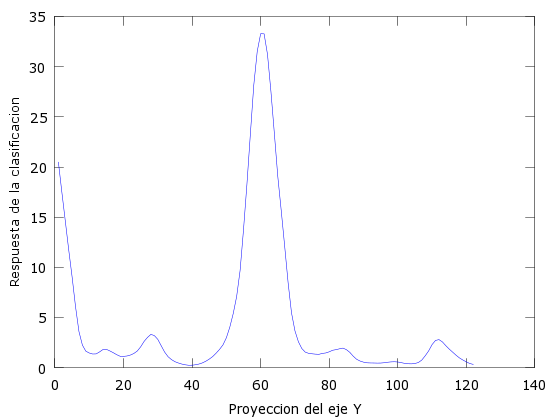
\includegraphics[scale=.4]{images/plots/svm7Y}
  \caption{\em  Proyección de ejemplo de resultados.A la izquierda, proyección en el eje x. A la derecha, proyección en el eje y. Arriba Adaboost. Abajo SVM}   
  \label{fig:pro7}
\end{figure}
\begin{figure}[H]
  \centering
  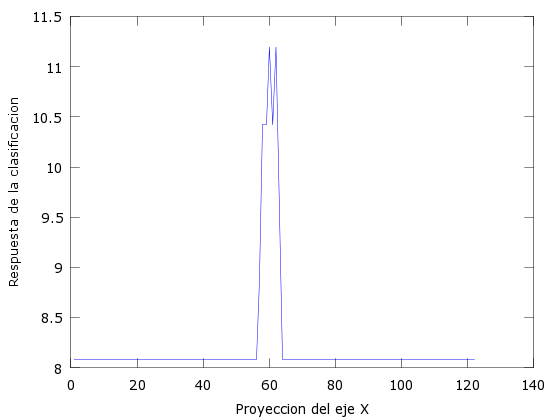
\includegraphics[scale=.4]{images/plots/boost8X}
  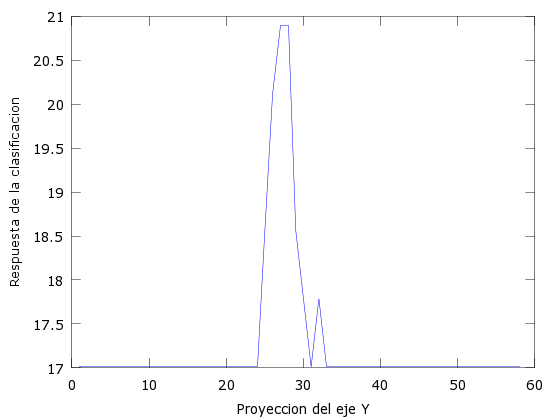
\includegraphics[scale=.4]{images/plots/boost8Y}
  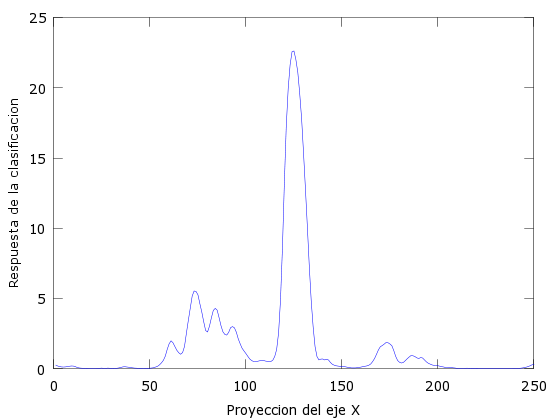
\includegraphics[scale=.4]{images/plots/svm8X}
  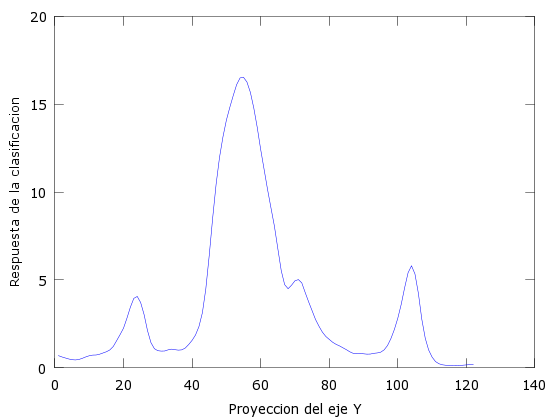
\includegraphics[scale=.4]{images/plots/svm8Y}
 \caption{\em  Proyección de ejemplo de resultados.A la izquierda, proyección en el eje x. A la derecha, proyección en el eje y. Arriba Adaboost. Abajo SVM}   
 \label{fig:pro8}
\end{figure}
